\documentclass
 [a4paper, 					% Papierformat
	11pt,							% Schriftgröße
	twoside,					% Seitenausrichtung auf gerade/ungerade Seitenzahl angepasst
	DIV=16,						% Aufteilung der Seite (s. KOMA-Skript-Dokumentation)
	BCOR=10mm,					% Bindungskorrektur: Zusätzlicher Rand auf der Innenseite
										% smallheadings, normalheadings, bigheadings: selbsterklärend
	chapterprefix, 		
	appendixprefix, 
	numbers=noenddot,
	plainfootsepline,	% setzt die für heading-Seiten (alle Seiten außer Kapitelanfangsseiten) 															
										% definierte Linie in der Fußzeile auch für plain-Seiten (Kapitelanfangsseiten)
	parskip=half,		% Absatz wird nicht eingerückt, dafür aber um eine halbe Zeile nach unten gerückt		
	bibliography=totoc,					
										% Literaturverzeichnis im Inhaltsverzeichnis aufgelistet
										% bibliography=totocnumbered dito, aber nummeriert
	listof=totoc,			% Tabellen- und Abbildungsverzeichnis im Inhaltsverzeichnis aufgelistet
										% listoftocnumbered dito, aber nummeriert
										% idxtotoc: Index im Inhaltsverzeichnis aufgelistet
	english,headinclude = true, %option was not given
	footinclude = false, %option was not given
	openany,          % no empty page before chapter
	]{scrbook}				% Dokumentklassen im KOMA-Skript: scrbook, scrartcl, scrreprt
%------------------------------------------------------------------------------------------------------
% ---- Kodierung ---- 
\usepackage[utf8]{inputenc}										
\usepackage{pifont} % ist nötig, um eingekringelte Zahlen schreiben zu können
										%(\ding{172}-\ding{211}, s. Table 188 der Datei Latex Symbols Dante)
%------------------------------------------------------------------------------------------------------
% ---- Sprache ----
\usepackage[T1]{fontenc} 				
\usepackage[english, ngerman]{babel}										
\addto\captionsenglish{\renewcommand{\figurename}{Figure}
											 \renewcommand{\tablename}{Table}}
\usepackage{csquotes}
%------------------------------------------------------------------------------------------------------
% ---- Farbdefinition ----
\usepackage[table]{xcolor}
										% Paket für farbigen Text -> xcolor statt color und table statt usename nötig für 										
										% farbig alternierende Tabellenzeilen dann \xdefinecolor statt \definecolor!
\usepackage{lmodern}

%		\xdefinecolor{DarkBlue}{RGB}{0,0,100}
%		\xdefinecolor{CoolBlue}{RGB}{6,96,120}
%		\xdefinecolor{CoolBlue2}{RGB}{6,96,143}
%		\xdefinecolor{CoolBlue3}{RGB}{5,111,166}
%		\xdefinecolor{LightBlue}{RGB}{157,193,211}
%		\xdefinecolor{Gray}{RGB}{100,100,100}

%  	\xdefinecolor{RWTHBlue}{RGB}{0,84,159} 
%  	\xdefinecolor{RWTHlightBlue}{RGB}{142,186,229}
%	 	\xdefinecolor{RWTHBlue}{RGB}{0,103,166} 
%		\xdefinecolor{RWTHlightBlue}{RGB}{119,158,201}
%		\xdefinecolor{RWTHRed}{RGB}{204,0,0} 
%		\xdefinecolor{Gray1}{RGB}{238,238,236}
%		\xdefinecolor{Gray2}{RGB}{211,215,207}
%		\xdefinecolor{Gray3}{RGB}{186,189,182}
%		\xdefinecolor{hellblau1}{rgb}{0.4666,0.7196,0.8882}
%		\xdefinecolor{hellblau2}{rgb}{0.6666,0.7196,0.8882}

% Alles s/w (fast)
	 	\xdefinecolor{RWTHBlue}{RGB}{0,0,0} 
	 	\xdefinecolor{myRWTHBlue}{RGB}{0,0,0} %{0,84,159} 
		\xdefinecolor{RWTHlightBlue}{RGB}{0,0,0} 
		\xdefinecolor{RWTHRed}{RGB}{0,0,0} %{0,51,153}  % now blue
		\xdefinecolor{Gray1}{RGB}{0,0,0} 
		\xdefinecolor{Gray2}{RGB}{0,0,0} 
		\xdefinecolor{Gray3}{RGB}{0,0,0} 
		\xdefinecolor{hellblau1}{rgb}{0,0,0} 
		\xdefinecolor{hellblau2}{rgb}{0,0,0} 
		
% Farben für Matlab-Listings
\xdefinecolor{hellgelb}{rgb}{1,1,0.85}     % Hintergrundfarbe
\xdefinecolor{colKeys}{RGB}{0,0,255}       % blau
\xdefinecolor{colIdentifier}{RGB}{0,0,0}	  % schwarz
\xdefinecolor{colComments}{RGB}{34,139,34} % gruen
\xdefinecolor{colString}{RGB}{160,32,240}  % violett

%------------------------------------------------------------------------------------------------------
% ---- Eigene Befehlsdefinitionen ----
\usepackage{xspace}
\usepackage{multirow}
\usepackage{titletoc}
\usepackage{xspace}
\usepackage{lscape}
\usepackage{bbold}
\usepackage{multicol}
\usepackage{siunitx}
\usepackage{lipsum}
% Referenzieren
\newcommand{\rfig}[1]{Fig.\,\ref{#1}}
\newcommand{\rapp}[1]{App.\,\ref{#1}}
\newcommand{\req}[1]{Eq.\,(\ref{#1})}
\newcommand{\rsec}[1]{Sec.\,\ref{#1}}      
\newcommand{\rchap}[1]{Chap.\,\ref{#1}} 
\newcommand{\rtab}[1]{Tab.\,\ref{#1}}  

% Short mathcal
\newcommand{\mc}[1]{\ensuremath{\mathcal{#1}}}
\newcommand{\mr}[1]{\ensuremath{\mathrm{#1}}}
\newcommand{\vsym}[1]{\ensuremath{\bm{#1}}}
% Shorthands
\newcommand{\tr}[0]{\ensuremath{\mathrm{tr}}\xspace}
\newcommand{\pqs}[0]{\ensuremath{\Ket{\psi}}\xspace}
\newcommand{\Ut}[0]{\ensuremath{U_t}\xspace}
\newcommand{\qp}[0]{\ensuremath{\mc{E}}\xspace}
\newcommand{\F}[0]{\ensuremath{\mc{F}}\xspace}
\newcommand{\IF}[0]{\ensuremath{1-\mc{F}}\xspace}
\newcommand{\ptm}[0]{\ensuremath{\mc{R}}\xspace}
\newcommand{\dif}[0]{\ensuremath{d}\xspace}
\newcommand{\sint}[3]{\ensuremath{\int#3 \! #1 \, \dif #2}}
\newcommand{\bsint}[3]{\ensuremath{\int#3 \! \dif #2 \, #1}}
\newcommand{\del}[0]{\ensuremath{\partial\xspace}}
\newcommand{\sts}[0]{S-T\textsubscript{0}\xspace}
\newcommand{\db}[0]{\ensuremath{\mr{\Delta}B}\xspace}
\newcommand{\dbz}[0]{\ensuremath{\mr{\Delta}B_z}\xspace}
\newcommand{\ddbz}[0]{\ensuremath{\delta \mr{ \Delta}B_z}\xspace}
\newcommand{\dt}[0]{\ensuremath{\mr{\Delta}t}\xspace}
\newcommand{\je}[0]{\ensuremath{J(\epsilon)}\xspace}
\newcommand{\jj}[0]{\ensuremath{J}\xspace}
\newcommand{\djj}[0]{\ensuremath{\deps}\xspace}
\newcommand{\epst}[0]{\ensuremath{\epsilon(t)}\xspace}
\newcommand{\eps}[0]{\ensuremath{\epsilon}\xspace}
\newcommand{\deps}[0]{\ensuremath{\delta \epsilon}\xspace}
\newcommand{\vecsig}[0]{\ensuremath{\vsym{\sigma}}\xspace}
\newcommand{\figlabel}[1]{\textbf{(#1)}}
\newcommand{\chim}[0]{\ensuremath{\chi}\xspace}
\newcommand{\dm}[0]{\ensuremath{\rho}\xspace}
\newcommand{\dv}[0]{\ensuremath{\mathbf{r}}\xspace}

\newcommand{\px}[0]{\ensuremath{\sigma_x}\xspace}
\newcommand{\py}[0]{\ensuremath{\sigma_y}\xspace}
\newcommand{\pz}[0]{\ensuremath{\sigma_z}\xspace}
\newcommand{\eye}[0]{\ensuremath{I}\xspace}
\newcommand{\ex}[1]{\ensuremath{\left\langle #1 \right\rangle}\xspace}
\newcommand{\nseg}[0]{\ensuremath{N_{\mathrm{seg}}}\xspace}
\newcommand{\ndbz}[0]{\ensuremath{N_{\dbz}}\xspace}
\newcommand{\nruns}[0]{\ensuremath{N_{\mathrm{runs}}}\xspace}
\newcommand{\dg}{\ensuremath{^\circ}}%
\newcommand{\thz}{\ensuremath{\theta = 0\dg}\xspace}
\newcommand{\thn}{\ensuremath{\theta = 90\dg}\xspace}
\newcommand*\conj[1]{\overline{#1}}
\newcommand*\mean[1]{\overline{#1}}
\newcommand{\ud}[0]{\ensuremath{\ket{\uparrow \downarrow}}\xspace}
\newcommand{\du}[0]{\ensuremath{\ket{\downarrow \uparrow}}\xspace}
\newcommand{\uu}[0]{\ensuremath{\ket{\uparrow \uparrow}}\xspace}
\newcommand{\dd}[0]{\ensuremath{\ket{\downarrow \downarrow}}\xspace}
\newcommand{\la}[0]{\ensuremath{\leftarrow}\xspace}

\newcommand{\ii}[0]{\ensuremath{\eye \otimes \eye}\xspace}
\newcommand{\ix}[0]{\ensuremath{\eye \otimes \px}\xspace}
\newcommand{\iy}[0]{\ensuremath{\eye \otimes \py}\xspace}
\newcommand{\iz}[0]{\ensuremath{\eye \otimes \pz}\xspace}
\newcommand{\XI}[0]{\ensuremath{\px \otimes \eye}\xspace}
\newcommand{\xx}[0]{\ensuremath{\px \otimes \px}\xspace}
\newcommand{\xy}[0]{\ensuremath{\px \otimes \py}\xspace}
\newcommand{\xz}[0]{\ensuremath{\px \otimes\pz}\xspace}
\newcommand{\yi}[0]{\ensuremath{\py \otimes \eye}\xspace}
\newcommand{\yx}[0]{\ensuremath{\py \otimes \px}\xspace}
\newcommand{\yy}[0]{\ensuremath{\py \otimes \py}\xspace}
\newcommand{\yz}[0]{\ensuremath{\py \otimes \pz}\xspace}
\newcommand{\zi}[0]{\ensuremath{\pz \otimes \eye}\xspace}
\newcommand{\zx}[0]{\ensuremath{\pz \otimes \px}\xspace}
\newcommand{\zy}[0]{\ensuremath{\pz \otimes \py}\xspace}
\newcommand{\zz}[0]{\ensuremath{\pz \otimes \pz}\xspace}

\newcommand{\x}[1]{\ensuremath{X_{\pi/2}^{(#1)}}\xspace}
\newcommand{\y}[1]{\ensuremath{Y_{\pi/2}^{(#1)}}\xspace}
\newcommand{\cn}[0]{\ensuremath{CNOT}\xspace}
\newcommand{\m}[1]{\ensuremath{M_{z}^{(#1)}}\xspace}
\newcommand{\algaas}{\ensuremath{\mr{Al_{0.3}Ga_{0.7}As}}}
\newcommand{\gaas}{\ensuremath{\mr{GaAs}}}




%ttfamily
\newcommand{\ttf}[1]{{\ttfamily #1}}
\newcommand{\parheading}[1]{\vspace{0.5em}{\noindent \sffamily \textbf{#1}}\vspace{0.25em}\\
}
% Große römische Zahlen im Fließtext: I durch \Roem{1}, V durch \Roem{5} usw.
\makeatletter 			% Den \catcode des at-Zeichens (»@«) auf 11 (letter) setzen. Nötig für Einlesen von Quellcodes.
\newcommand{\Roem}[1]{%
                      \textsc{%           % für Kapitölchen
                              \@Roman{#1}% Das Argument als roemische Ziffer
                              }%\          % Ein normalgroßes Leerzeichen, wichtig bei nonfrenchspacing
                     %\ignorespaces       % Keine weiteren Leerzeichen ausgeben.
                      }
\makeatother 				% Den \catcode des at-Zeichens (»@«) auf 12 (other) setzen. 
%------------------------------------------------------------------------------------------------------
% ---- Inhaltsverzeichnis ----
\setcounter{tocdepth}{3} 
										
%------------------------------------------------------------------------------------------------------
% ---- Seitenlayout ----
% ---- Gliederung und Kapitelüberschriften ----
\setcounter{secnumdepth}{3} 
										% Bestimmt, bis zu welcher Schachtelungstiefe eine Nummerierung der Überschriften 										 
										% erfolgt.Standardmäßig ist 2 eingestellt, d.h. Kapitel- Abschnitts- und 															% Unterabschnittsüberschriften erhalten eine fortlaufende Nummer.
										% Mögliche Werte sind:
											% -1 	keine Überschrift wird nummeriert
											% 0 	Kapitelüberschriften (oder Abschnittsüberschriften im article.sty) werden 											
											%     nummeriert
											% 1 	die beiden höchsten Ebenen werden nummeriert
											% 5 	alle Überschriften werden nummeriert. (Die Werte 2, 3, 4 ergeben die 												  	
											%     Zwischenwerte...) 
%\renewcommand*{\raggedsection}{} 
										% KOMA-Script setzt Überschriften von \chapter bis \subparagraph in linksbündigem 										
										% Flattersatz mit hängendem Einzug. Verantwortlich ist dafür die Anweisung 														
										% \raggedsection, die vordefiniert ist als: \let\raggedsection\raggedright
										% Die Anweisung \raggesection kann mit \renewcommand*{\raggedsection}{} oder 													
										% \let\raggedsection\relax so umdefiniert werden, dass Überschriften im Blocksatz 										
										% stehen.
% \setkomafont{chapter}{\color{RWTHBlue}\bfseries\rmfamily\Large}
										% Einstellungen der Schrift der Kapitelüberschrift im KOMA-Skript
										% (Schriftfarbe, fetter Text, Schriftart, Schriftgröße)
										% Die Schriftformatierung der Kapitelüberschriften gebe ich in \titleformat ein 											
										% paar Zeilen weiter unten schon an, weshalb sie an dieser Stelle überflüssig ist.	
% \setkomafont{chapter}{\color{RWTHBlue}\bfseries\sffamily\Large}
\setkomafont{section}{\bfseries\sffamily\Large\color{RWTHBlue}}			
\setkomafont{subsection}{\bfseries\sffamily\large\color{RWTHBlue}}
%\setkomafont{subsubsection}{\bfseries\sffamily\large\color{RWTHBlue}}
										
\usepackage{titlesec}
										% beliebige Formatierung von Überschriften, für den folgenden Befehl notwendig										
 \titleformat{\chapter}[display]
 						 {\vspace*{-2cm}\sffamily\bfseries\color{RWTHBlue}\fontsize{22}{22}\selectfont}
             {\filleft{\chaptertitlename} {\thechapter}}
             {0,5ex}
             {{\color{RWTHBlue}\titlerule}\vspace{2ex}} 
             []
             
 \titleformat{\part}[display]
 						 {\vspace*{-2cm}\sffamily\bfseries\color{RWTHBlue}\fontsize{27}{27}\selectfont}
             {Part {\thepart}}
             {0,5ex}
             {{\color{RWTHBlue}\titlerule}\vspace{2ex}} 
             []
										% \titleformat{Überschriftenklasse}[Absatzformatierung]
										%             {Textformatierung}
										%             {Kapitelnummer/Label mit Angaben zur Schriftformatierung (kann freigelassen werden)}
										%             {Abstand zw. Kapitelnummer/Label und Überschriftentext}
										%             {Code vor der Überschrift}
										%             [Code nach der Überschrift]
										% {\part, \chapter, \section,...}[hang, block, display, runin, leftmargin, rightmargin, drop, wrap, frame]
										% {\vspace bestimmt horizontale Position, negativer Abstand schiebt alles nach oben;
										%  Schriftart, fettgedruckt, Schriftfarbe, Schriftgröße}
										% {\chaptertitlename erzeugt "Chapter", Leerzeichen, \thechapter erzeugt die entsprechende Kapitelnummer}
										% {ob der Abstand vertikal oder horizontal gemessen wird, hängt von der Abstatzformatierung ab (display -> vertikal); 										%  ex entspricht Höhe des Buchstaben x; dieses Feld darf nicht frei gelassen werden -> soll kein Platz zwischen 
										%  Kapitelnummer und Überschrift gelassen werden, muss man 0ex/0cm/... einsetzen}
										% {erzeugt schwarze Linie}
										% []
											% Mit dem Format display wird das Label in einen eigenen Absatz gesetzt, mit dem Format hang steht es auf gleicher 
												% Höhe wie die Linie der Kopfzeile, weitere Bedeutungen: 
												% http://ctan.org/tex-archive/macros/latex/contrib/titlesec/titlesec.pdf
											% \fontsize{size}{skip} ändert die Schriftgröße (size) und den Zeilenabstand (skip); um diesen Befehl wirksam zu 
											% machen, ist \selectfont nötig -> \fontsize{size}{skip}\selectfont
											% \filleft: rechtsbündiger Text (\filright: linksbündiger Text, \filinner: Text immer am äußeren Seitenrand)
											
% ---- Zeilenabstand ----
\usepackage{setspace} 
\onehalfspace				

% ---- Kopf- & Fußzeilen ----

% (vgl. zur Seitenaufteilung ftp://ftp.dante.de/pub/tex/macros/latex/contrib/koma-script/scrguide.pdf, Seite 231)

\usepackage{scrpage2}
										% für Verwendung von Kopf- und Fußzeilen
										% definiert eigene plain- und heading-Stile: scrplain und scrheadings
									  	 % (plain = Seitenzahl in Fußzeile, Kopfzeile leer,
									  	 %  headings erlaubt komplexere Einstellungen)
									  	 % \pagestile{scrheadings} scrplain muss nicht separat aufgerufen werden, da scrheadings das ohnehin tut 
										   
\clearscrheadings
\clearscrplain			% löscht voreingestellte Stile
	
	
	
% Eigene Einstellungen:



%\setlength{\headheight}{1.1\baselineskip}
                       % LaTeX gibt mir in meinem speziellen Fall folgende Warnung aus: 
                       	% Package scrpage2 Warning: seems you are using a very small headheight. If you get overfull \vbox warnings at 
                       	% almost every page, you should increase headheight e.g. writing \setlength{\headheight}{1.1\baselineskip} into 
                       	% the preambel of your document.
                       % Dies ist aber nicht zwingend nötig.
\automark[chapter]{section}
										% \automark[<rechte Seite>]{<linke Seite>}
										% die rechte Seite wird in der Kopf-/Fußzeile mit \rightmark, die linke Seite mit \leftmark aufgerufen

% Following options changed, original ones commented out
\setkomafont{pagenumber}{\normalfont \sffamily} 
%\setkomafont{pagenumber}{\normalfont \sffamily \bfseries \color{RWTHBlue}}     
										% Einstellungen der Schrift der Seitenzahl im KOMA-Skript
										% Standardfont, Schriftart, fetter Text, Schriftfarbe
										
\setheadsepline{1pt}[{\color{RWTHBlue}}]
										% \setheadsepline[Länge]{Dicke}[Befehle] erzeugt Linie unter dem Header
										% \setheadtopline[Länge]{Dicke}[Befehle] erzeugt Linie über dem Header
%\setfootsepline{1pt}[{\color{RWTHBlue}}]
										% \setfootsepline[Länge]{Dicke}[Befehle] erzeugt Linie über der Fußzeile
										% \setfoottopline[Länge]{Dicke}[Befehle] erzeugt Linie unter der Fußzeile
\lehead[]{\pagemark}
\rehead[]{\sffamily \upshape \color{RWTHBlue} \rightmark}
                    % Kopfzeile, linker Seitenrand bei geraden Seitenzahlen -> äußerer Rand
                    % [steht auf Kapitelseiten in der Kopfzeile/Fußzeile (Eigentlich gibt man hier an, was man da beim pagestyle "plain" 	
                    %  haben möchte, das ist auch der Seitenstil, der bei Seiten mit neuen Kapitelüberschriften gewählt wird)]
                    % {steht auf allen anderen Seiten in der Kopfzeile/Fußzeile}
                      % []{Schriftart, aufrecht, Schriftfarbe, Einfügen des Kapitelnamens}
\rohead[]{\pagemark}
\lohead[]{\sffamily \upshape {\color{RWTHBlue} Section \leftmark}}
										% Kopfzeile, rechter Seitenrand bei ungeraden Seitenzahlen -> äußerer Rand
										% [steht auf Kapitelseiten in der Kopfzeile/Fußzeile (Eigentlich gibt man hier an, was man da beim pagestyle "plain" 	
                    %  haben möchte, das ist auch der Seitenstil, der bei Seiten mit neuen Kapitelüberschriften gewählt wird)]
                    %	{steht auf allen anderen Seiten in der Kopfzeile/Fußzeile}
                      % []{Schriftart, aufrecht, Schriftfarbe, Einfügen eines eigenen Textes (also nur auf Seiten, auf denen kein neues 
                      %    Kapitel beginnt)}
%\ofoot[{\sffamily \color{RWTHBlue} \pagemark}]{{\sffamily \color{RWTHBlue} \pagemark}}
										% Fußzeile, äußerste Textbox (mittlere Textbox: \cfoot, innerste Textbox: \ifoot)
 										% [steht auf Kapitelseiten in der Kopfzeile/Fußzeile (Eigentlich gibt man hier an, was man da beim pagestyle "plain" 	
                    %  haben möchte, das ist auch der Seitenstil, der bei Seiten mit neuen Kapitelüberschriften gewählt wird)]
                    % {steht auf allen anderen Seiten in der Kopfzeile/Fußzeile}
 											% [Schriftart, Schriftfarbe, Einfügen der Seitenzahl]{Schriftart, Schriftfarbe, Einfügen der Seitenzahl}
%\ifoot[\sffamily \upshape {\color{RWTHBlue}High-Fidelity Qubit Gates for Two-Electron Spin Qubits}]
%      {\sffamily \upshape {\color{RWTHBlue}High-Fidelity Qubit Gates for Two-Electron Spin Qubits}}
										% Fußzeile, innerste Textbox (s.o.)
										% [steht auf Kapitelseiten in der Kopfzeile/Fußzeile(Eigentlich gibt man hier an, was man da beim pagestyle "plain" 	
                    %  haben möchte, das ist auch der Seitenstil, der bei Seiten mit neuen Kapitelüberschriften gewählt wird)]
                    % {steht auf allen anderen Seiten in der Kopfzeile/Fußzeile}
                    	% [Schriftart, aufrecht, Schriftgröße, Text in entsprechenden Farben]
                    	% {Schriftart, aufrecht, Schriftgröße, Text in entsprechenden Farben}
                    		% \vert erzeugt einen senkrechen Strich (|), muss in mathematischer Umgebung stehen
\pagestyle{scrheadings} 
										% Ruft selbst definierte Einstellungen für Kopf- und Fußzeilen auf.


										
% \automark[section]{chapter}											% \automark[<rechte Seite>]{<linke Seite>} im Header
										% Beispiele: 
										% \ohead{\pagemark}           % Oben außen: Seitenzahlen
										% \ihead{\headmark} 					% Oben innen: Setzt Kapitel und Section automatisch
										% \rehead{\leftmark} 					% Oben links: Chapter ???
										% \lohead{\rightmark}				  % Oben rechts: Section ???
										% \cfoot[\pagemark]{} 				% Mitte unten: Seitenzahlen bei plain
										%\cfoot[]{\pagemark} 					% Mitte unten: Seitenzahlen bei headings




%\begin{landscape}
%...
%\end{landscape}
% ---- Bilder ----

\usepackage{graphicx} 	
										% Einbinden von Bildern	
										% automatische Konvertierung von .eps nach .pdf
%
\usepackage{wrapfig}
\usepackage[sf,small,nooneline,FIGTOPCAP]{subfigure} 
															
\usepackage[format=plain]{caption}
\usepackage{placeins} 						
\usepackage[]{subfigure}
%\usepackage{svg}
\usepackage[rflt]{floatflt} 
									
\makeatletter										
	\newcommand\figcaption{\def\@captype{Figure}\caption}
	\newcommand\tabcaption{\def\@captype{Table}\caption}
\makeatother
										
\addtokomafont{captionlabel}{\color{myRWTHBlue}\sffamily\small\bfseries}							
\addtokomafont{caption}{\color{black}\sffamily\small}									
											
%------------------------------------------------------------------------------------------------------
% ---- Tabellen ----
%\usepackage[table]{xcolor} s.o. bei Farbdefinitionen!
                    % erlaubt Verwendung von Farben in Tabellen
                     		% \cellcolor{color} 		Einfärben von einzelnen Tabellenzellen
                     		% \rowcolor{color} 			Einfärben von Zeilen										
                     		%			-> \rowcolors{<starting row>}{<odd rows colour>}{<even rows colour>}
                     		%												Erzeugt abwechselnd gefärbte Zeilen
                     		% \hiderowcolors				Färbt Zeilen NICHT mehr ein
                     		% \showrowcolors				Färbt Zeilen wieder ein
                     		% \columncolor{color}		Einfärben von Spalten
\usepackage{booktabs}
										% erlaubt die Verwendung von \toprule, \midrule und \bottomrule zum Erzeugen dicker Linien

\usepackage{longtable}
                    % Ermöglicht Einfügen von Tabellen, die sich über mehrere Seiten erstrecken
%------------------------------------------------------------------------------------------------------
% ---- Aufzählung ----
\usepackage{enumerate}
\renewcommand{\labelitemi}{$\diamond$}
 										
%------------------------------------------------------------------------------------------------------
% ---- Fußnote ----                     		
\interfootnotelinepenalty=10000	
										% Verhindert das Aufsplitten einer Fußnote auf 2 Seiten.																	
%------------------------------------------------------------------------------------------------------
% ---- Referenzieren ----
%\usepackage[numbers,sort&compress]{nat}   
%                    % Wenn dieses Paket mit den angegebenen Optionen geladen wird, werden die 														
%                    % Referenzen sortiert: [12,1,5,6,4] -> [1,4-6,12] 
%\bibliographystyle{apsrev} % revtex4

\usepackage[backend=bibtex,
	   % sortlocale=de_DE,
    	natbib=true,
			bibencoding=auto,			
		  style=phys, %numeric-comp,
		  sortcites = true,
			arxiv = abs,
			doi = false,
			url = true,
			isbn = false,
			minnames=1,
			maxcitenames=2,
			maxbibnames=99,
			backref=true,
			hyperref=true]{biblatex}		%% Lädt das Biblatex Paket und definert den Style
%\usepackage[citestyle=plain, bibstyle=plain, minnames=1, maxnames=2, hyperref=true]{biblatex}
%% Styles: numeric für Zahlen in eckigen Klammern [1]
%\renewcommand*{\nameyeardelim}{\space}
%\defbibnote{urlinfo}{Stand der Onlineverweise: 22. August 2012.}%\today.}
% Infos zu Biblatex http://mirror.informatik.uni-mannheim.de/pub/mirrors/tex-archive/macros/latex/exptl/biblatex/doc/examples/01-introduction.pdf
%\defbibheading{head}{\section{Literaturverzeichnis}}
%\addbibresource{bibliography/MA.bib}

% et. al in italics
\renewbibmacro*{name:andothers}{% Based on name:andothers from biblatex.def
  \ifboolexpr{
    test {\ifnumequal{\value{listcount}}{\value{liststop}}}
    and
    test \ifmorenames
  }
    {\ifnumgreater{\value{liststop}}{1}
       {\finalandcomma}
       {}%
     \andothersdelim\bibstring[\emph]{andothers}}
    {}}
\addbibresource{./library.bib}

\usepackage[colorlinks=true, linkcolor=RWTHRed, citecolor=RWTHRed, menucolor=myRWTHBlue, linktocpage=false, breaklinks=false, urlcolor=black, %backref=page, 
pdfpagelayout=TwoColumnRight]{hyperref}
										  												
%\renewcommand*{\backref}[1]{}
%	\renewcommand*{\backrefalt}[4]{%
%	\ifcase #1 %
%	%
%\or
%Cited on page #2.%
%\else
%Cited on pages #2.%
%\fi
%}						 
%\renewcommand{\figureautorefname}{figure}
                    % Bei Verwendung von Babel:
                    \addto\extrasenglish{\def\figureautorefname{figure}}
%\newcommand{\subfigureautorefname}{\figureautorefname}
										% erzeugt bei der Verwendung von \autoref beim Verweis auf eine Subfigure die Bezeichnung "figure" 
										\addto\extrasenglish{\def\subfigureautorefname{\figureautorefname}}
%\renewcommand{\tableautorefname}{table}
                    % Bei Verwendung von Babel:
                    \addto\extrasenglish{\def\tableautorefname{table}}										
%\renewcommand{\sectionautorefname}{Section}
										% erzeugt bei der Verwendung von \autoref beim Verweis auf eine Subsection die Bezeichnung "section"
										% Bei Verwendung von Babel: 
										\addto\extrasenglish{\def\sectionautorefname{section}}
%\renewcommand{\subsectionautorefname}{Section}
										% erzeugt bei der Verwendung von \autoref beim Verweis auf eine Subsection die Bezeichnung "section"
										% Bei Verwendung von Babel: 
										\addto\extrasenglish{\def\subsectionautorefname{\sectionautorefname}}
%\renewcommand{\subsubsectionautorefname}{\sectionautorefname}
										% erzeugt bei der Verwendung von \autoref beim Verweis auf eine Subsubsection die Bezeichnung "section"
										% Bei Verwendung von Babel: 
										\addto\extrasenglish{\def\subsubsectionautorefname{\sectionautorefname}}
%\renewcommand{\subsubsubsectionautorefname}{\sectionautorefname}
										% erzeugt bei der Verwendung von \autoref beim Verweis auf eine Subsubsubsection die Bezeichnung "section"
										% Bei Verwendung von Babel: 
										\addto\extrasenglish{\def\subsubsubsectionautorefname{\sectionautorefname}}
%\renewcommand{\equationautorefname}{equation}
										% erzeugt bei der Verwendung von \autoref beim Verweis auf eine Subsubsubsection die Bezeichnung "section"
										% Bei Verwendung von Babel: 
										\addto\extrasenglish{\def\equationautorefname{equation}}
\newcommand{\autoeqref}[1]{\hyperref[#1]{\equationautorefname~(\ref*{#1})}}			
                    % Setzt Formelnummer in Klammern																	
% Springer-Verlag-Konvention:
%\addto\extrasenglish{\def\figureautorefname{Fig.}}
%\addto\extrasenglish{\def\chapterautorefname{Chap.}}
%\addto\extrasenglish{\def\sectionautorefname{Sect.}}
%\addto\extrasenglish{\def\pageautorefname{p.}}
%\usepackage{cleveref}
                 	  % Muss nach Hyperref geladen werden!
                 	  % Referenzieren mittels \cref (Kleinschreibung) und \Cref(Großschreibung)
                 	  % Mehrere Verweise können durch Kommata getrennt angegeben werden: \cref{eq:1,eq:2,eq:3} -> equation 1 to 3
                 	  % Aufbrechung einer Zusammenfassung durch zusätzliches Komma: \cref{eq:1,eq:2,eq:3,,eq:4} -> equation 1 to 3 and 4
                 	  % options:
                 	  %		sort: Sortiert Verweislisten, aber fasst sie nicht zusammen.
                 	  % 	compress: Fasst zusammenhängende Verweise zusammen, aber sortiert die Liste nicht.
                 	  %		nosort: Sortiert Verweislisten nicht und fasst sie auch nicht zusammen.
                 	  %		sort&compress: Sortiert Verweislisten und fasst zusammenhängende Verweise zusammen. (Default)
                 	  % !! Schreibt "footnote" statt "equation". Synchronisieren mit hyperref!?
                 	  % !! Verschiebt im Anhang alle Bilder!?
%Beispiel für Satzanfang:
%\hyperref[labelName]{Section~\ref{labelName}} % Section wird groß geschrieben
% Referenzieren auf eine bestimmte Textstelle:
										% \autopageref{page:Textstelle}
										% Die Textstelle muss gekennzeichnet sein durch
										% \phantomsection\label{page:Textstelle}
%------------------------------------------------------------------------------------------------------
% ---- Mathematik und Sonderzeichen ----
\usepackage[OMLmathsfit]{isomath}
                     % Verwendung von mathsfit zum Kursivschreiben in einer serifenlosen Matheschrift
\usepackage{amsmath, % Einbinden mathematischer Symbole
						amssymb, % stellt Sonderzeichen für den Mathematikmodus bereit
%           latexsym,% Einbinden von Latex-Symbolen
            textcomp,% stellt das copyright-zeichen \textcopyright berreit
            upgreek, % ermöglicht aufrechte Schreibweise von griechischen Buchstaben, z.B. \mu -> \upmu
            bm,		   % ermöglicht fette UND kursive Schreibweise in Mathemodus über \bm
%           isomath, % wird vom Paket fixmath gebraucht zur Verwendung von \mathbfit (s.o.)
            fixmath  % Verwendung von mathbfit zum Kursiv- und Fettschreiben von griechischen Großbuchstaben
                    }
              
% Übersicht über Befehle für serifenlose Matheschrift:
% \mathsf            % serifenlose Schrift im Mathemodus (aufrecht) -> Auch für Zahlen benutzen! In kursiver Schreibweise werden die klein!
% \mathsfit          % serifenlose, kursive Schrift im Mathemodus
% \mathboldsans      % serifenlose, fette, kursive Schrift im Mathemodus  
% \bm{\mathsf{}}     % serifenlose, fette Schrift im Mathemodus
%------------------------------------------------------------------------------------------------------
% ---- Anhang ----
%------------------------------------------------------------------------------------------------------
% ---- Literatur- und Bilderverzeichnis ----
% \usepackage{multibib}
										% Möglichkeit, mehrere Literaturverzeichnisse zu erstellen
										% Funktioniert leider noch nicht
%  \newcites{lit}{Bibliography}
	% \newcites{bi}{List of Figures}
										% \newcites{irgendwas}{Titel des ersten Verzeichnisses} ermöglicht es, im Text den \cite-Befehl, mit dem man auf 
										% BibTeX-Einträge zugreifen und zitieren kann, zu erweitern zu \citeirgendwas:
												% \cite{Literaturquelle1} oder \citebi{Bildquelle1}
										% Anleitung: http://www.macuser.de/forum/f51/latex-man-dokument-146261/
												% Erstellen einer BibteX-Datei mit den Literatureinträgen, z.B. Literature.bib und Figures.bib
												% Diese Befehle rufen am Ende des Dokuments die Einträge in Literature.bib bzw. Figures.bib auf, die mit 
												% \citeirgendwas mit dem ersten Verzeichnis verknüpft wurden:	
														%\bibliographystylelit{unsrt}
														%\bibliographylit{Zwischenbericht1Literatur_bib}		
														%\bibliographystylebi{unsrt} 
														%\bibliographybi{Zwischenbericht1Bilder_bib}
												% ALTERNATIVE: TeXnicCenter verwenden, Projekt erzeugen mit aktueller Datei als Hauptdatei auswählen, bei BibTex 
												% verwenden ein Häkchen setzen, 1x pdf kompilieren, 1x Ausgabe -> BibTex, 2x pdf kompilieren
												% Quellen, die nicht zitiert werden, aber in den Verzeichnissen erscheinen sollen, werden mit \nocite oder 
												% \nociteirgendwas verknüpft
												% In der Eingabeaufforderung:
														% latex dokument -> Kompilieren
														% bibtex irgendwas -> Dieser Befehl erzeugt eine Datei irgendwas.aux, die mit BibTeX kompiliert werden muß
																% Hier also: bibtex lit und bibtex bi
														% bibtex Literatur.bib -> Kompilierung mit bibtex
																% Hier also: bibtex Literature.bib und bibtex Figures.bib
                          	% 2x latex dokument
%\bibliographystyle{unsrt}                     	
%------------------------------------------------------------------------------------------------------
% ---- To-do-Liste ----
\usepackage[colorinlistoftodos % Erzeugt eine farbige Box vor den To-Do-Listeneinträgen
						,disable   % Entfernt alle To-Do-Einträge
						]{todonotes}
												% \todo[options]{todo text} erstellt eine To-Do-Notiz am Textrand
													% Options:
													% bordercolor=color			Rand der Notizbox
													% backgroundcolor=color	Hintergrundfarbe der Box
													% linecolor=color				Farbe der Linie, die Box und Textstelle verbindet
													% line/noline           Erzeugt die Verbindungslinie (default) oder lässt sie weg.
													% inline/noinline				Setzt die Kommentarbox in den Text oder an den Rand.
													% \todo[caption={Short note}]{Text}
													%												Erlaubt Erstellung eines langen Kommentars, bei dem "Short note" in der To-Do-Liste 
													%                       erscheint und der Text an gewünschter Stelle im Text.
												% \missingfigure{text} erstellt eine Platzhalter für das fehlende Bild einschließlich Text
													% \missingfigure[figwidth=6cm]{Testing a long text string}
													%												Erstellt Bild-Platzhalter der angegebenen Breite.
													% \missingfigure{Testing a long text string}
													%												Setzt Platzhalter über komplette Textbreite.
													% \begin{wrapfigure}{r}[2cm]{6cm}
													%  \missingfigure[figwidth=6cm]{Add a test image \ldots}
													% \end{wrapfigure}
													%												Setzt Platzhalter in Wrapfigure-Umgebung.
												% \listoftodos erstellt eine To-Do-Liste
												% \todototoc in der Präambel erzeugt den Eintrag der To-Do-Liste im Inhaltsverzeichnis
												
												% Meine Farbcodierung:
													% To do!: 							default
													% Offene Fragen:				backgroundcolor=green!40
													% Zusatzinfos:					backgroundcolor=blue!20!white
%------------------------------------------------------------------------------------------------------
% ---- includeonly ----
%\includeonly{Titelseite,
             %Vorlage-Thesis-Introduction,
             %Vorlage-Thesis-Theory_of_PCM, 
             %Vorlage-Thesis-TitaniumDioxide,
             %Vorlage-Thesis-TheFerroelectric_transition_in_GeTe,
             %Thesis-Motivation3,
             %scintificInstruments,
             %Thesis-experimental_results,
             %Thesis-Outlook,
             %Thesis-TheoBack, 
             %Thesis-ExpRes,
             %Thesis-Summary,
             %Thesis-Outlook,
             %Vorlage-Thesis-Appendix}
%-------------------------------------------------------------------------------------------------------             
             
%-------------------------------------------------------------------
%- RWTH Aachen II. Physikalisches Institut C - Prof. Hendrik Bluhm -
%- Projekt: Simulation and Optimization of multi qubit quantum dots-			
%- Bachelorarbeit Rene Otten ---------------------------------------
%- Titel: Simulation and Optimization of multi qubit quantum dots---
%- Betreuer: Pascal Cerfontaine ------------------------------------
%-------------------------------------------------------------------
%- Template by Tim Leonard und Pascal Cerfontaine-------------------
%-------------------------------------------------------------------
\usepackage{epstopdf}
\usepackage{epsfig}
\usepackage{bbm}
\usepackage{braket}
\usepackage{geometry}
\usepackage{here} 
\usepackage[numbered,framed]{matlab-prettifier}
\usepackage[final]{pdfpages}
\lstset{%
  style           	  = Matlab-editor,
  basicstyle       	  = \mlttfamily\small,
  escapechar       	  = ",
  mlshowsectionrules 	= true,
  mlscaleinline			= false,
}
%/////////////////////////////////////////////////////////////////////////////////////////////////////////////////////////////
%/////////////////////////////////////////////////////////////////////////////////////////////////////////////////////////////


%\titlecontents{chapter}[0pt]{\addvspace{3pt}}{\contentsmargin{0pt}
%\bfseries\makebox[0pt][r]{\normalsize\thecontentslabel\enspace}\normalsize}
%{\contentsmargin{0pt}\large}{\bfseries\hfill\contentspage}[\addvspace{1pt}] %\bfseries\hfill\contentspage




%\usepackage{perpage}
%\MakeSorted{figure}
%\MakeSorted{table}

\begin{document}	

\def\blurb{%
 
\Large Master's Thesis in Physics\\[0.8em]
\footnotesize presented to\\
\normalsize The Faculty of Mathematics, Computer Science \\and Natural Sciences
\normalsize at RWTH Aachen University\\[0.8em]
\normalsize Department of Physics, Quantum Technology Group\\
\normalsize Oktober 2017\\[0.8em]

\footnotesize supervised by\\
\normalsize Prof. Hendrik Bluhm, PhD\\
Pascal Cerfontaine, M.Sc. RWTH
 
  }

\def\clap#1{\hbox to 0pt{\hss #1\hss}}%
\def\ligne#1{%
  \hbox to \hsize{%
    \vbox{\centering #1}}}%
\def\haut#1#2#3{%
  \hbox to \hsize{%
    \rlap{\vtop{\raggedright #1}}%
    \hss
    \clap{\vtop{\centering #2}}%
    \hss
    \llap{\vtop{\raggedleft #3}}}}%
\def\bas#1#2#3{%
  \hbox to \hsize{%
    \rlap{\vbox{\raggedright #1}}%
    \hss
    \clap{\vbox{\centering #2}}%
    \hss
    \llap{\vbox{\raggedleft #3}}}}%

\makeatletter
  \let\oldcaption\caption
  \renewcommand{\caption}[2][]{%
  \oldcaption[#1]{\textbf{#1} #2}
  }
\makeatother

\thispagestyle{empty}\vbox to .9\vsize{%
  \vss
  \vbox to 1\vsize{%
    
    
    \vspace{10cm}\ligne{\Huge Exchange Mediated Two-Qubit Gates for Two-Electron Spin Qubits}
    \vspace{5mm}
    \ligne{\Large by René Otten}
    \vfill
   
    \vspace{5mm}
\haut{}{\blurb}{}
   
    }%
  \vss
  }
  
  
%/////////////////////////////////////////////////////////////////////////////////////////////////////////////////////////////
%/////////////////////////////////////////////////////////////////////////////////////////////////////////////////////////////  

\listoftodos
%\pagenumbering{Roman}

%----------------------------------------------------------------------------------------------------------------------------------------	

% ---- Befehle, die hinter \begin{document} stehen müssen (?): ----

 %\renewcommand*\thesubfigure{\colorbox{RWTHlightBlue}{\color{black}\sffamily\small\textbf{\alph{subfigure}}}\hfill}
						% Funktioniert weder in der Präambel noch im Dokument selbst!!!
										% \renewcommand[\Befehl]{Anzahl der Parameter}{Inhalt} definiert einen Befehl um
										% Die Sternchenversion \renewcommand* nimmt keine Parametertexte an, die Absatzumbrüche enthalten. Es ist 		
										% sozusagen eine Kurzversion, die bevorzugt verwendet werden sollte. LaTeX kann so evtl. Fehler besser behandeln.
										% Umdefinierung des Befehls \thesubfigure: Erzeugt hellblaue Box mit schwarzer Schrift, serifenfreie 
										% Schriftart, kleine Textgröße, fettgedruckt, alphanummerische Nummerierung beginnend mit "a" 
														% \alph{Zähler} gibt den Wert des angegebenen Zählers als lateinischen Kleinbuchstaben aus
														% (Alternativen: \Alph (lateinische Großbuchstaben), \arabic (arabische Ziffer), 
														% \roman (römische Zahl in Kleinbuchstaben), \Roman (römische Zahl in Großbuchstaben)
														% \hfill definiert einen horizontalen Zwischenraum, der jede beliebige Länge annehmen kann


%----------------------------------------------------------------------------------------------------------------------------------------	
%----------------------------------------------------------------------------------------------------------------------------------------
%----------------------------------------------------------------------------------------------------------------------------------------	

% Festlegung der Seitenzahlzählweise

%\pagenumbering{roman}	  
										% \pagenumbering{Art} legt die Art der Seitenzählung fest. Ab dem Auftreten dieses Befehls erscheinen Seitennummern in 
										% der angegebenen Darstellungsart; dabei steht arabic für arabische Zahlen, roman für römische Zahlen und alph für 
										% lateinische Buchstaben. Roman und Alph stehen für die entsprechenden Großbuchstaben (s.o.). 
										
%----------------------------------------------------------------------------------------------------------------------------------------	

% Sprachauswahl

\selectlanguage{ngerman}   
										% \selectlanguage{language} schaltet zwischen den zuvor geladenen Sprachpaketen (\usepackage[english, ngerman]{babel})
										% um. 
										
%----------------------------------------------------------------------------------------------------------------------------------------
\frontmatter
% ---- Titelseite ----
%\include{1_1_titlepage/titlepage}
%----------------------------------------------------------------------------------------------------------------------------------------
%----------------------------------------------------------------------------------------------------------------------------------------	
%----------------------------------------------------------------------------------------------------------------------------------------
 
\cleardoublepage    % Beendet eine Seite und erzwingt auf den nachfolgenden Seiten die Ausgabe aller Gleitobjekte (z.B. Abbildungen), die 
										% bislang definiert, aber noch nicht ausgegeben wurden. Dieser Befehl fügt, falls nötig, eine leere Seite ein, sodaß 	
										% die nächste Seite nach den Gleitobjekten eine ungerade Seitennummer hat. 
\thispagestyle{empty}
										% \thispagestyle{Art} legt die Art des Seitenformats für eine einzelne Seite fest. 
										% plain:      zentrierte Seitennummer am Seitenfuß
										% empty:      keinerlei Kopf oder Fuß 
										% headings:   Kopfzeile aus der Seitennummer und der Überschrift des laufenden Abschnitts
										% myheadings: erlaubt es, den Seitenkopf selbst mit den \markright- und \markboth-Befehlen zu definieren. 
										

%----------------------------------------------------------------------------------------------------------------------------------------	

% Sprachauswahl

\selectlanguage{english}   
										% \selectlanguage{language} schaltet zwischen den zuvor geladenen Sprachpaketen (\usepackage[english, ngerman]{babel})
										% um. 								
											
%----------------------------------------------------------------------------------------------------------------------------------------	
%----------------------------------------------------------------------------------------------------------------------------------------
%----------------------------------------------------------------------------------------------------------------------------------------	
% ---- Abstract ----

%/////////////////////////////////////////////////////////////////////////////////////////////////////////////////////////////
%/////////////////////////////////////////////////////////////////////////////////////////////////////////////////////////////

\vspace*{\fill}

\begin{center}
\begin{minipage}{0.75\textwidth}

\begin{center}
{\bfseries\sffamily\Large\color{RWTHBlue} Abstract}
\end{center}
\begin{singlespace}
\lipsum[1]


\end{singlespace}
\end{minipage}
\end{center}

\vspace*{\fill}

%/////////////////////////////////////////////////////////////////////////////////////////////////////////////////////////////
%/////////////////////////////////////////////////////////////////////////////////////////////////////////////////////////////

%----------------------------------------------------------------------------------------------------------------------------------------
 										
%------------------------------------------------------------------------------------------------------
% ---- Inhaltsverzeichnis ----
\begingroup
	\hypersetup{linkcolor=RWTHBlue}
	\tableofcontents 
\endgroup
										% Das Einbetten der Table of Contents in diese Gruppe ermöglicht SCHWARZE Einträge ins Inhaltsverzeichnis, obwohl
										% die Einträge Hyperlinks darstellen und deshalb in der Farbe der definierten Linkcolor gedruckt werden würden.
%------------------------------------------------------------------------------------------------------
%------------------------------------------------------------------------------------------------------
%------------------------------------------------------------------------------------------------------
% ---- List of figures ----
%\listoffigures
%------------------------------------------------------------------------------------------------------
% ---- List of tables ----
%\listoftables
%------------------------------------------------------------------------------------------------------
\mainmatter
\pagenumbering{arabic}
%------------------------------------------------------------------------------------------------------
% ---- Chapter 1: Introduction ----
\chapter{Introduction}
\label{chap:intro}

\section{Motivation}
Peaking with the recent release of the IBM quantum experience interest in quantum computing, or more general quantum information processing, has recently been on the rise. In addition to the scientific community the general public has become increasingly aware leading to programs like the EU quantum effort. Further industry leaders like IBM, Google and Microsoft have shown great interest sparking major collaborations with university all around the globe. 

Quantum information processing holds the potential to revolutionize modern computing by employing basic quantum mechanical principles namely superposition, tunneling and entanglement. This would allow for efficient simulation of quantum mechanical systems, leading to the field of quantum simulation, but also provide an exponential speedup with some more common task like prime factorization using Shors (quantum) algorithm. 
In this so called \textit{Second Quantum Revolution} artificial quantum mechanical systems are employed to solve the tasks mentioned above.

The incredible potential held by quantum information processing has led to a zoo of different approaches trying to create qubits, which are the fundamental building blocks making up a quantum computer. The most important ones that are still actively researched are ion trap qubits, superconducting qubits and electron spin qubits without there being a clear winner. 
On the theoretical side there  has been extensive work on the conditions for a working quantum computer leading to the so called DiVincenzo criteria:
\begin{enumerate}
    \item A scalable physical system with well characterised qubits.
    \item The ability to initialise the state of the qubits to a simple fiducial state.
    \item Long relevant decoherence times.
    \item A “universal” set of quantum gates.
    \item A qubit-specific measurement capability.
\end{enumerate}
To also allow for quantum communication two more criteria have to be added:
\begin{itemize}
    \item The ability to interconvert stationary and flying qubits.
    \item The ability to faithfully transmit flying qubits between specified locations.
\end{itemize}
(see \rfig{fig:layout}). 
At the time of this thesis high fidelity single and two qubit gates have been shown with many different approaches and material systems, while first multi qubit systems have been explored.
In this thesis I will focus on two-electron spin qubits in GaAs, one of the most mature semiconductor based systems, with coherence times exceeding $\si{200.\micro s}$



\section{Goal}
In this thesis, I will take some of the essential steps on the way towards an experimental realization of exchange driven two qubit gates in GaAs in order to perform Gate optimization based on tuning protocols previously employed in our group. 
High Fidelity two qubit gates are a necessary requirement for a quantum computer in any material system. With its high coherence times, all electrical control and straight forward fabrication GaAs is the perfect material system for the development of methods and algorithms that can be transferred to other material systems later.


\section{Outline}

 

 
%------------------------------------------------------------------------------------------------------
% ---- Chapter 2: 
\chapter{Introduction to Semiconductor Based Electron Spin Qubits}
\label{chap:motivation}
\section{Qubit}
A qubit, or generally speaking a quantum mechanical two level system 
$ \ket{\Psi} = \alpha \ket{0} + \beta \ket{1} $, where $\alpha, \beta \in \mathbb{C}$ and $|\alpha|^2 + |\beta|^2=1$ can be expressed as
\begin{equation}
    \ket{\Psi}=\cos \left( \frac{\theta}{2} \right) \ket{0} + \exp(i \phi) \sin \left( \frac{\theta}{2} \right) \ket{1} \quad \text{where}\;  \phi, \theta \in \mathbb{R}
\end{equation}
when a global phase is neglected. This allows us to visualize this pure state as a point on the so called Bloch Sphere.

However, information about the exact quantum mechanical state can be lost to the environment leading to the definition of mixed states.  Mixed states are statistical ensembles of different quantum states and can be expressed via the density matrix 
\begin{equation}
    \dm = \sum_i p_i \ket{\psi_i}\bra{\psi_i}
\end{equation}
For a 2-dimensional system we can use the Pauli-Matrices to rewrite $\dm$ in terms of $\px$, $\py$ and $\pz$
\begin{equation}
    \dm= \frac{1}{2}(\eye+\vsym{r} \cdot \vecsig)
\end{equation}
where $|\vsym{r}|\le 1$. In fact $|\vsym{r}|= 1$ only for pure states and $|\vsym{r}|< 1$ for mixed states. \cite{Feynman1957}

 \begin{figure}[htbp]\centering
     \centering
     \includegraphics[width=0.35\textwidth]{./pictures/dummy}
     \caption{PICTURE BLOCH SPHERE}
     \label{fig:bloch_sphere}
 \end{figure}

Ignoring interactions with the environment for now, we can model the time evolution of a quantum mechanical system, and therefore a qubit, using the unitary time evolution operator $U(t,t_0)$. $U$ acts on the initial state of the system given by $\ket{\psi_0}$ leading us to, $\ket{\psi(t,t_0)}=U(t,t_0)\ket{\psi_0}$, the state at the time $t$. Using the Hamiltonian $H(t)$ we can calculate $U(t,t_0)$ 
\begin{equation}
U(t,t_0)=\mc{T}\exp \left( - \frac{i}{\hbar} \int_{t_0}^t H(t') dt'  \right),
\end{equation}
using the time-ordering operator. 
For qubits the time evolution can in general be explained by rotations on the Bloch sphere, making for a very intuitive picture of qubit operations. Many of these concepts have been in use for some in NMR experiments, but can be easily applied to all kinds of qubits be it semiconductors, superconductors, NV centers or ion traps.

For two qubits, however, this simple picture breaks down. Of course we can express the individual qubits on their respective Bloch spheres, but since the interaction between the two becomes important, this can not depict the full information of the system. MORE?

\section{Quantum Dots}
Quantum dots are the predominant way to create semiconductor based qubits. A quantum dot is a system confining electrons in all the directions.

Confinement in one direction is usually archived by the growth of suiting heterostructures such as AlGaAS-GaAs or Si-SiGe combination (see REF) forming a two dimensional electron gas. Confinement in the remaining two directions is achieved by placing gate electrodes on top of the heterostructure. These allow for the creation of quantum dots, as well as for the control of tunneling to source and drain regions within the 2DEG. Further, so called plunger gates can shift the chemical potential of the quantum dot effectively controlling its population.

Interesting characteristics arise when the transport through a quantum dot is measured as a function of the plunger gate voltage. Assuming that the tunnel barriers to source and drain are clearly defined and transparent enough to allow for tunneling on a realistic timescale transport can be observed whenever one of the discrete dot energy levels is between the source and drain chemical potential. This assumes that a small bias voltage is applied between source and drain. Sweeping the gate voltage will lead to a oscillatory behaviour of the current REF. 

Since the energy levels of the dot are not only sensitive to changes in the gate voltage but also to charges nearby a quantum dot can be used as a very sensitive means of measuring charge REF. A quantum dot used in this capacity is often referred to as sensing dot or single electron transistor (SET). 

\begin{figure}[htbp] 
  \centering
     \subfigure[]{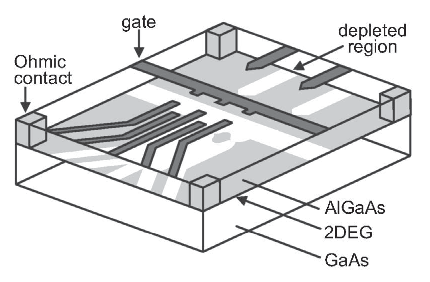
\includegraphics[width=0.49\textwidth]{./pictures/quantumdot1}}
   \subfigure[]{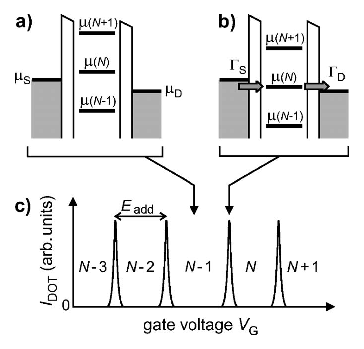
\includegraphics[width=0.49\textwidth]{./pictures/QuantumDot}}
  \caption{}
  \label{fig:quantumdots}
\end{figure}

 
\section{Heterostructure}
The heterostructures we use for our experiments is shown in PICTURE. They consist of a GaAs substrate on top of which a $\algaas \ $ layer is grown by molecular beam epitaxy (MBE). This layer contains Si-doping which provides charge carriers. These carriers accumulate at the $\algaas$/GaAs interface, where due to the band offset of the two materials a triangular quantum well is formed. The electron in this well create a two dimensional electron gas (2DEG) since they are confined in growth direction. 
The 2DEG is contacted by gold/germanium ohmic contacts which are fabricated in the Helmholz Nano Facility \cite{HNF}. This allows for control of the electrochemical potential of the 2DEG.
The heterostructure is topped off with a thin GaAs cap, on top of which metal electrodes are fabricated by electron beam lithography
These so called gates can be used to deplete the 2DEG selectively underneath the pattern by applying negative bias voltages. A possible gate design is shown in PICTURE.This procedure allows for the precise creation of dot regions with good control of the electron population within the dots.

\begin{figure}[htbp]\centering
     \centering
     \includegraphics[width=0.50\textwidth]{./pictures/Heterostructure}
     \caption{PICTURE Heterostructure}
     \label{fig:bloch_sphere}
 \end{figure}
 

\section{S-T0 Qubits}
The original proposal from Loss and DiVincenzo used individual spins in a semiconductor heterostructure as qubits. While viable for example in Silicon, this approach has a couple of inherent disadvantages in GaAs mainly caused by the perturbations due to the nuclear spin bath surrounding the qubits.
This problem can be mitigated using a double quantum dot with two spins in a external magnetic field, where the $m_z=0$ subspace of the system is used for computation. This approach has been successfully employed in many experiments and is proven to reach long coherence times in excess of $200\;\mr{\mu s}$.
Additional advantages are the option to control the qubit all electrically be changing the detuning and thus the exchange interaction between the two spins.
Straightforward spin to charge conversion.
MORE ADVANTAGES AND DIFFERENCES
200 mus Time
Single Shot Readout
Universal Control
Two  Qubit Gates 
DiVincenzo Criteria Backref





For an $\sts$ qubit the gates are used to form a double well potential, trapping exactly two electrons. An additional external magnetic field of the order of a couple $\si{100.mT}$ is applied in plane, separating of the $m_z=\pm1$ states $\ket{T_+}=\uu$ and $\ket{T_-}=\dd$ energetically. The remaining states in the $m_z=0$ subspace are then used as the computational basis states REF
\begin{align}
    \ket{0}&=\ket{S}=\frac{1}{\sqrt{2}}(\ud-\du) \\
    \ket{1}&=\ket{T_0}=\frac{1}{\sqrt{2}}(\ud+\du).
\end{align}
The degeneracy between the two computational states is lifted on the one hand by the exchange interaction $J$ and on the other hand by the magnetic field difference $\dbz$ between the dots.
$\dbz$ arises from the electron spins within the GaAs. Naturally these would cause a random difference in the magnetic field at the dot locations. However by using controlled spin flips the magnetic field gradient can be tuned to be within a few MHz of the desired values. Nevertheless control of $\dbz$ remains slow and the nuclear spins have to be "pumped" repeatedly in between measurements as the only remain stable for short amounts of time due to diffusion REFS.

The exchange interaction $J$ gives the second control axis for \sts qubits. It can be controlled via the detuning between two dots which is directly related to the voltage applied to the gate electrodes. Empirically, a exponential dependence
\begin{equation}
    J(\eps)=J_0 \exp \left( \frac{\eps}{\eps_0} \right)
\end{equation}
has been found to best describe the relation of the exchange interaction and the detuning. The resulting Hamiltonian for one qubit is then given by 

\begin{equation}
    H=\frac{\hbar J(\epsilon)}{2}\sigma_z + \frac{\hbar B_z}{2} \sigma_x.
\end{equation}

Using these two control axes universal control of \sts qubits in GaAs has been shown. A basic control cycle is depicted in \rfig{fig:controlcycle}. 

\begin{figure}[htbp]\centering
     \centering
     \includegraphics[width=1\textwidth]{./pictures/computationalcycle}
     \caption{PICTURE BLOCH SPHERE}
     \label{fig:controlcycle}
 \end{figure}

\begin{figure}[htbp] 
  \centering
     \subfigure[]{\includegraphics[width=0.49\textwidth]{./pictures/dummy}}
     \subfigure[]{\includegraphics[width=0.49\textwidth]{./pictures/dummy}}
   
  \caption{}
  \label{fig:cable}
\end{figure}


\section{Exchange Only Two Qubit System}
In theory the number of quantum dots which can be placed next to each other is only limited by fabrication. 

\begin{figure}[htbp]\centering
     \centering
     \includegraphics[width=.5\textwidth]{./pictures/gl005_SEM_electrons_small}
     \caption{PICTURE BLOCH SPHERE}
     \label{fig:controlcycle}
 \end{figure}
 
Computational Subspace

Coherent Leakage

Possible Gate design



\section{Previous Work}
\subsection{Single Qubit Gates}

Masterarbeit Pascal

PRL Paper

Bootstrap Tuning Paper

\subsection{Experimental Work on Two Qubit Gates in GaAs}

Harvard work on capacitivly coupled Qubits





%------------------------------------------------------------------------------------------------------
% ---- Chapter 3: 
\chapter{Theory}
\section{Qubit Description}
In the $\{ \ket{S},\ket{T_0} \}$ Basis the Hamiltonian is most commonly written as (CITE HANSON) written as
\begin{equation}
    H=\frac{\hbar J(\epsilon)}{2}\sigma_z + \frac{\hbar B_z}{2} \sigma_x.
\end{equation}

However it might be convenient, especially for computational purposes to rewrite the Hamiltonian in the $\{\ud,\du \}$ 
\begin{equation}
    H=\frac{\hbar J(\epsilon)}{2}\px + \frac{\hbar B_z}{2} \pz.
\end{equation}
such that the idle axis i.e. when the exchange interaction is turned points in the $z$-direction.
Pictures: Structure, Gates, Computational Cycle
\subsection{Exchange Only Two Qubit System}
For our two qubit system we want to exchange couple for quantum dots, resulting in two $\sts$ qubits, with an additional exchange coupling and magnetic field gradient in between. In order to model this system we start with an generic $N$ electron Heisenberg Hamiltonian
\begin{equation}
    H(t)=\mu \sum_{n=1}^N B_n(t) \pz^n + \frac{1}{4} \sum_{\langle i,j \rangle} J_{ij}(t)(\vecsig ^i \cdot \vecsig ^j - \eye).
\end{equation}
Since the experimentally accessible variables are $J_{ij}$ and $\db_{ij}=B_j-B_i$ we can rewrite $H$ in these terms for the case $N=4$ to
\begin{align}
    H(t)  &=  B_\mr{G}             [\pz^{(1)} + \pz^{(2)} + \pz^{(3)} + \pz^{(4)} ]  \nonumber\\
          &+ \frac{\db_{12}(t)}{8} [-3\pz^{(1)} + \pz^{(2)} + \pz^{(3)} + \pz^{(4)} ]\nonumber \\
          &+ \frac{\db_{23}(t)}{4} [-\pz^{(1)} - \pz^{(2)} + \pz^{(3)} + \pz^{(4)} ] \nonumber\\
          &+\frac{\db_{34}(t)}{8}  [-\pz^{(1)} - \pz^{(2)} - \pz^{(3)} +3 \pz^{(4)} ] \\
          &+\frac{J_{12}(\epsilon_{12}(t))}{4} (\vecsig ^1 \cdot \vecsig ^2 - \eye) \nonumber\\
          &+\frac{J_{12}(\epsilon_{23}(t))}{4} (\vecsig ^2 \cdot \vecsig ^3 - \eye) \nonumber\\
          &+\frac{J_{12}(\epsilon_{34}(t))}{4} (\vecsig ^3 \cdot \vecsig ^4 - \eye). \nonumber
\end{align}

Again using the $m_z=0$ subspace for computation we choose the basis to
\begin{align}
\ket{00} &= \ud \ud  \nonumber\\
\ket{01} &= \ud \du \nonumber\\
\ket{10} &= \du \ud \nonumber\\
\ket{11} &= \du \du .
\end{align}
However, unlike the one qubit system we now obtain two leakage states, namely $\uu \dd$ and $\dd \uu$ that are not split off energetically by the external magnetic field. This allows for coherent manipulation in and out of the leakage subspace.


\section{Fidelity Measures}
The is a rather large number of different measures of "Fidelity" that is used in literature. While all have their place and can usually be used interchangeably it is important to understand the subtle differences and restrict oneself to only one to avoid any confusion. Here I would like to introduce the most important ones which will be used throughout this thesis.

The state fidelity is used to characterize the distance of two states represented by the density matrices $\dm_1$ and $\dm_2$ and is defined by CITE
\begin{equation}
\F_\text{state}(\dm_1,\dm_2)=\tr \sqrt{\dm^{1/2}_1 \dm_2 \dm^{1/2}_1}.
\end{equation}
In case one of the two states is pure (e.g. $\dm_1$) in form of a state vector $\ket{\psi}$, $\F_\text{state}$ becomes
\begin{equation}
\F_\text{state}(\ket{\psi},\dm_2)=\tr \sqrt{\bra{\psi} \dm_2 \ket{\psi}},
\end{equation}
therefore the state fidelity can be interpreted as the overlap of the two states $\ket{\psi}$ and $\dm_2$.

However, we are usually interested in the Fidelity of a noisy quantum process, $\qp$, implementing a perfect unitary operator $\Ut$. Of course, we could simply apply both $\Ut$ and $\qp$ to an arbitrary initial state $\ket{\psi}$ and use REF. In order to gain Independence from the initial state however we can choose one of two options. Firstly we could introduce the minimum fidelity
\begin{equation}
\F_\text{min}(\Ut,\qp)=\min_{\pqs} \F(\Ut \pqs, \qp(\pqs \bra{\psi})).
\end{equation}
This gives a worst case estimate of the fidelity of an operation $\qp$.
Alternatively we can average overall possible initial states
\begin{equation}
\mean{\F}(\Ut,\qp)=\int \F(\Ut \pqs, \qp(\pqs \bra{\psi}))^2 d\psi.
\label{eq:avgfid}
\end{equation}
We can relate this fidelity measure to another one, that is defined differently.
The entaglement fidelity, $\F_e$, is defined via a pure state $\ket{RQ}$, where the quantum operation $\qp$ only acts on one half of the system, e.g. on $Q$ and leaves the other half untouched. $\F_e$ is than defined as
\begin{equation}
\F_e(\ket{RQ} \bra{RQ},\qp(\ket{RQ} \bra{RQ}))=\F_\text{state}(\ket{RQ} \bra{RQ},(\eye_R \otimes \qp)(\ket{RQ} \bra{RQ}))^2.
\end{equation}
Since we included a square in the definition of \ref{eq:avgfid}, we can now directly relate this to the entanglement fidelity via
\begin{equation}
\mean{\F}(\Ut,\qp)=\frac{d\F_e(\Ut,\qp)+1}{d+1}.
\end{equation}
where $d$ is the dimension of the qubit system, e.g. for one qubit ($d=2$) this results in $1-\mean{\F}=\frac{2}{3}(\IF_e)$ and for two qubits ($d=4$) this leads to $1-\mean{\F}=\frac{4}{5}(\IF_e)$.
CITE

\section{Pauli Transfer Matrix}
As it has been previously demonstrated on single qubits gates, we want to implement an self consistent, iterative tune up of our gates that can be implemented in real experiments. For single qubit gates the decomposition of errors in axis and angle errors is straight forward. However in the two qubit space this simple and intuitive picture is somewhat lost. Therefore we need to find an alternative, more general way to quantify our gate errors that ideally is still somewhat intuitive and allows us to employ our iterative tuneup protocol for a two qubit system.

A very useful tool in this context is the Pauli-Transfer-Matrix (PTM) as defined by
\begin{equation}
    (\ptm_\qp)_{ij}=\frac{1}{d}\tr{(P_i \qp(P_j))},
\end{equation}
where $P_i$ is given by the set of Pauli Matrices and unity, $\{\eye, \px,\py,\pz\}^{\otimes n}$.
Intuitively a state given by its density matrix, $\rho$, is decomposed in the basis $\vec{P}$ such that
\begin{equation}
\dm = \frac{1}{d} \vec{p} \cdot \vec{P}.
\end{equation}
The same is done to the final state after the process $\dm_\text{f}=\qp(\dm)$ resulting in $\vec{p}_\text{f}$. The PTM is the matrix that connects $\vec{p}_\text{f}$ and $\vec{p}$ by \begin{equation}
    \vec{p}_\text{f}=\ptm \vec{p}
\end{equation}
This allows for very easy and intuitive analysis of the gates as can be seen here (CITE QPT Transmon)

\section{Two Qubit Bootstrap Tomography}
% S=    | 1o1 1oX 1oY 1oZ |
%       | Xo1 XoX XoY XoZ |
%       | Yo1 YoX YoY YoZ |
%       | Zo1 ZoX ZoY ZoZ |
For the two dimensional qubit system $\vec{P}$ is given by the set
\begin{equation}
\{\eye, \px,\py,\pz\}^{\otimes 2}=
\begin{Bmatrix}
\ii & \ix & \iy & \iz \\
\XI & \xx & \xy & \xz \\
\yi & \yx & \yy & \yz \\
\zi & \zx & \zy & \zz 
\end{Bmatrix}.
\end{equation}
Again $\vec{p}$ will be the corresponding coeffiecents of $\dm$ of a given state. We need to construct sequences of the gates
$U_A = X_{\pi/2}$, $U_B = Y_{\pi/2}$ and $U_C = CNOT$ that allow us to determine all errors on $\vec{p}$, with $\vec{p}_0$ being the coefficients for a perfect gate. 

Therefore, we calculate the expectation value of our two measurement operators  $M_{i(j)} \in \{ \zi, \iz \}$ given by
\begin{equation}
S_j =\tr{(M_{i(j)}\dm_j)}
\end{equation}
where  $\dm_j = U_j \dm_0 U_j^\dagger$. Assuming we have near perfect gates we linearize around $\vec{p}_0$ and find gates that fullfil
\begin{equation}
S(\vec{p})-S(\vec{p}_0) =\frac{\dif \vec{S}}{\dif \vec{p}}(\vec{p}-\vec{p}_0)
\end{equation}
by determining the Jacobian $\frac{\dif \vec{S}}{\dif \vec{p}}$ numerically. From the soulutions we select the matrix $\frac{\dif \vec{S}}{\dif \vec{p}}$ with the best condition number since we want to use $\vec{S}$ for optimizing our gates in the experiment.
The resulting sequences are shown in \rtab{tab:sequences}. We apply each of the sequences in our simulation to the ground state $\ket{00}$. Sequences 1 to XX are designed to yield the measurement outcome 0 as we are maximally sensitive at this point. Sequences XX to ZZ are used to include decoherence. Without decoherence these would give the result one. If decoherence is included they will be modified with a factor $(1-\frac{16}{15}(\IF_e))$ as explained in REF.
  


\section{Depolarizing Channel}
The simplest model to  estimate the effect of noise on a quantum state is the depolarizing channel. In this view, the qubit is depolarized meaning placed in a completely mixed state $\eye/2$ with a probability $p$. Accordingly the qubit is left untouched remaining in its initial state with a probability $1-p$.
This operation can be written as
\begin{equation}
    \qp (\rho)=\frac{p\eye}{2}+(1-p)\rho
    \label{eq:depol2d}
\end{equation}
or for a qubit system of arbitrary dimension
\begin{equation}
    \qp (\rho)=\frac{p\eye}{d}+(1-p)\rho
\end{equation}
where $d$ is the dimension of the qubit space, e.g. for a two qubit system $d=4$. For a single qubit a depolarizing channel can be thought of a uniform contraction of the bloch sphere.
A common pitfall when modeling depolarizing channels is the parametrization of the probability $p$. Using the equation
\begin{equation}
    \frac{\eye}{2}=\frac{\rho+\px \rho \px + \py \rho \py +\pz \rho \pz }{4}
\end{equation}
we can rewrite \ref{eq:depol2d} 
\begin{equation}
    \qp (\rho)=\left(1-\frac{3p}{4}\right)\rho+\frac{p}{4}(\rho+\px \rho \px + \py \rho \py +\pz \rho \pz )
\end{equation}
which is often written as
\begin{equation}
    \mathcal{E} (\rho)=(1-q) \rho+\frac{q}{3}(\rho+\px \rho \px + \py \rho \py +\pz \rho \pz )
\end{equation}
using $q=\frac{3p}{4}$. Often the depolarizing channel is introduced without any indication which parametrization is used.
In order to model decoherence quickly when knowing only $\F_e$ we need to estimate the minimum state fidelity of a depolarizing channel starting with a pure state $\ket{\psi}$
\begin{equation}
\F_{state}(\ket{\psi}\bra{\psi},\qp(\ket{\psi}\bra{\psi}))=\sqrt{\bra{\psi} \left(\frac{p\eye}{d}+(1-p)\ket{\psi}\bra{\psi} \right) \ket{\psi}}
\end{equation}
leading us to
\begin{equation}
\mean{\F} \approx \F^2_{state} = 1-\frac{d-1}{d}p.
\end{equation}
Using REF for a two qubit system this leads to $\mean{\F}=1-\frac{3}{4}p$ and finally
\begin{equation}
\F_e=1-\frac{15}{16}p.
\end{equation}
We can use this result to estimate the effect of decoherence on our measurement, $\langle(\pz \otimes \eye )\rangle$ for
\begin{align}
\langle(\pz \otimes \eye)\rangle &=\tr{[\qp(\rho) (\pz \otimes \eye)]} \\
                     &=\underbrace{\frac{p}{d}\, \tr{(\pz \otimes \eye)}}_{=0}+(1-p) \, \tr (\rho (\pz \otimes \eye))\\
                     &=(1-p)\langle(\pz \otimes \eye)\rangle_{\text{w/o noise}}\\
                     &=(1-\frac{16}{15}(\IF_e)) \langle(\pz \otimes \eye)\rangle_{\text{w/o noise}}.
\end{align}
where we used $d=4$ in the last step. This allows us to model the effect of decoherence on our measurement simply by multiplying a factor to our measurement outcome without noise. 


%------------------------------------------------------------------------------------------------------
% ---- Chapter 4: 
\chapter{Device Testing}

In this chapter I will discuss the gate layouts we used during this project as well as explain the selection process we follow in order to find samples, fullfilling the requirements for the implementation of two qubit gates (CHAPTERS).
\section{Sample Design}
In order to do exchange mediated two qubit gates, we have to modify existing, proven gate design to our requirements. In particular the distance between qubit one and two has to be reduced greatly in order to allow for the exchange coupling to be the dominat interaction. A comparison between our layout and previous ones is shown in \rfig{fig:layout_comp}.
\begin{figure}[htbp] 
  \centering
     \subfigure[]{\includegraphics[width=0.2\textwidth]{./pictures/dummy}}
     \subfigure[]{\includegraphics[width=0.2\textwidth]{./pictures/dummy}}
  \caption{}
  \label{fig:layout_comp}
\end{figure}
Each of the gates is supposed to control a specific parameter of the two qubit system, be it the tunnel coupling between to dots, or the overall position of one dot. In order to given an overview over the specific purposes of different gates an illustrated version of the gate layout is shown in \rfig{fig:colorful_gatelayout}.

\begin{figure}[htbp]\centering
     \centering
     \includegraphics[width=0.2\textwidth]{./pictures/dummy}
     \caption{}
     \label{fig:colorful_gatelayout}
 \end{figure}
 
\section{Testing Process}
In order to select a sample, where a sufficient number of gates is working, we have to perform a number of somewhat standardized measurements. I will provide a brief overview adapted from tim Botzem (REF) at this point. A more detailed "checklist" is provided in \rapp{app:testing}.

\section{Pinch Off Measurements}
One of the most important pre-characterization measurements are so called Pinch Off measurements. The sample is contacted as shown in PICTURE. WE apply a bias voltage across two ohmic contacts and measure the resulting current using a Lock-In amplifier (Settings are included in Appendix REF). We than use at least two gates to create a narrow channel by applying negative voltages. This will slowly reduce the conductance across the sample until it vanishes completely. The point at which the current reaches zero is called pinch off voltage and gives an indication of the distance of the gates forming the channel. Examples are shown in PICTURE.
Using information on the symetry of the gate design we can easily evaluate the state of the device without resorting to any complicated measurements.

\section{Kurt Measurements}
Broke
\subsection{Future Gate Designs}
Design for future generations
%------------------------------------------------------------------------------------------------------
% ---- Chapter 5: 
\chapter{RF Readout Part}
\label{chap:setup}
In this chapter I will take a closer look at qubit readout via RF reflectometry measurements. \rsec{sec:RF_paper} is a draft for a paper discussiong in detail effects that various parts of a standart RF setup have. In \rsec{sec:RFcalib} I will discuss how we used this to tune our own two qubit readout circuit.

\section{High Frequency Lock in Techniques for Qubit Readout}
\label{sec:RF_paper}

\section{PAPERDRAFT Simulation of High Frequency Read Out}
Simple Schematic of ReadOut 
Formula
Some simulation
Medford Thesis
\includepdf[pages=-]{./chapters/APS}


\section{Calibration of Read Out circuit}
\label{sec:RFcalib}


% ---- Paper Draft 1: 


\chapter{Paperdraft Gate Simulations}

\includepdf[pages=-]{./chapters/APS}
% ---- Paper Draft 2: 


\chapter{Paperdraft Bootstrap Tune Up}

\includepdf[pages=-]{./chapters/APS}
%------------------------------------------------------------------------------------------------------
% ---- Chapter 8: 
\chapter{Summary and Outlook}
\label{chap:summary}

%------------------------------------------------------------------------------------------------------
\backmatter										
%------------------------------------------------------------------------------------------------------
% ---- Appendix + Bibliography ----
\pagenumbering{roman}
\begin{appendix}

	\chapter{Appendices}					% erzeugt Kapitel ohne Nummerierung sowie den entsprechenden Eintrag ins Inhaltsverzeichnis;
															% führt bei meinem Layout dazu, dass auf der Kapitelanfangsseite des Anhangs nicht über dem Strich noch 
															% einmal Appendix steht -> Appendix ist nur "Pseudokapitel"
	\refstepcounter{chapter}		% beginnt mit der Nummerierung eines Pseudokapitels, weist also dem Appendix-"Kapitel" eine Nummerierung zu, 
															% so dass die Sections im Inhaltsverzeichnis unter A.1, A.2 usw. aufgelistet werden
	
	%\pagenumbering{Roman}   
											        % \pagenumbering{Art} legt die Art der Seitenzählung fest. Ab dem Auftreten dieses Befehls erscheinen Seitennummern in 
											        % der angegebenen Darstellungsart; dabei steht arabic für arabische Zahlen, roman für römische Zahlen und alph für 
											        % lateinische Buchstaben. Roman und Alph stehen für die entsprechenden Großbuchstaben (s.o.). 
	
	\renewcommand{\thesection}{\Alph{section}}
	\numberwithin{equation}{section}
	\numberwithin{figure}{section}
	\numberwithin{table}{section}
	
%/////////////////////////////////////////////////////////////////////////////////////////////////////////////////////////////
%/////////////////////////////////////////////////////////////////////////////////////////////////////////////////////////////
 
										% \pagenumbering{Art} 
\section{Device Layouts}
\subsection{002}
\subsection{003}
\subsection{005}

\section{Device Testing Procedure}
\label{app:testing}

\begin{enumerate}
\item{In order to contact the device, an interposer chip is glued onto a PCB using GE varnish. It is essential to cover the entire part of the PCB that is supposed to take the interposer with the glue and prevent the formation of air bubbles as these can lead to problems with wire-bonding.}
\item{Next the sample is glued onto the interposer chip. Again formation of air pockets should be avoided. Additionally care has to be taken in order to prevent the glue to get onto the bond pads on the sample or the interposer side.}
\item{At this point the sample should be grounded at all times! This includes a shorting PCB in the DC connection port as well as shoring caps on the RF lines.}
\item{Now the sample and interposer can be wire-bonded to the PCB. The connection between PCB and interposer should be done first to ensure proper grounding.}
\item{From this point forward the sample should be transported on ESD safe foam and in an ESD save compartment. }
\item{At this point the lines in the ,,dicke Bertha'' or any other setup used should be checked for their connection and their resistance to ground.}
\item{Once proper functionality of the setup is ensured, we can mount our sample to the dipstick. Special care should be taken when connecting SMPM connectors as they have a tendency to break. Since there are more RF lines on the PCB then in the setup, a single line can be connected to multiple ones on the PCB.}
\item{Now room temperature measurements can be performed. Using a Keithley 2400 source meter unit, we can check the connection to our ohmics and our gates. The Keithley is set to $ \si{0.V}$} with a compliance of $\si{1.\micro\ampere}$. At this point the diode behaviour of the gates, as well as the linear resistance of the ohmic contacts could be probed.
However, just by connecting the Keithley and taking the respective port from ground, we can gain an indication of weather we are connected to an ohmic contact or a gate. For efficiency, long measurements are usually omitted at this point. (Make sure that the output of the Keithley is ON! Otherwise it is left floating and the voltage is not defined.) 
\item At this point the sample can be cooled down to $\si{4K}$ and the measurements continued here. It has been useful in the past to mark the ohmic contacts with tape on the breakout box.
\item Once "special-measure" is set up using the setup-script, Lock-In and DecaDAC can be connected to the Breakout Box. Make sure, that the fridge is grounded either by the Lock-In Output or a separate ground! Only disconnect the ground line if the Lock-In is connected.
\item At this point Pinch-Off measurements using the automation script can be performed. Detailed description can be found in REF.
\item Given that the sensing dots can be pinched off, tuning measurements for the RF readout cirucit can be performed at this point. Power levels of $\si{50.dBm}$ are be sufficent, and should not be exceeded to prevent damage to the sample. More details can be found HERE.

\end{enumerate}



\newpage
\section{Bootstrap Sequences}

\begin{table}[htbp]
        \centering
        \begin{tabular}{l | l l l l|r} \hline 
            $j$ &$U_j$  &&&&   $M_{i(j)}$\\ \hline \hline
       
            1&$\cn $&$\la \x{1}$   &&&   $\m{1}$ \\ 
            2& $\x{1} $&$\la \cn$   &&&   $\m{1}$ \\ 
            3&$\cn $&$\la \y{1}$   &&&   $\m{1}$ \\ 
            4&$\y{1}$&$\la \cn$   &&&   $\m{1}$ \\
            5&$\cn $&$\la \x{2}$    &&&   $\m{2}$ \\
            6&$\cn $&$\la \y{2}$    &&&   $\m{2}$ \\
    %
            7&$\x{1} $&   $\la \cn$ & $\la \x{1}$  &&   $\m{1}$ \\ 
            8&$\x{1} $&   $\la \cn$ & $\la \y{1}$  &&   $\m{1}$ \\  
            9&$\y{1} $&   $\la \cn$ & $\la \x{1}$  &&   $\m{1}$ \\ 
            10&$\x{1} $&   $\la \x{2}$ & $\la \cn$  &&   $\m{2}$ \\ 
            11& $\y{1} $&   $\la \cn$ & $\la \y{1}$  &&   $\m{1}$ \\  
            12&$\y{1} $&   $\la \y{2}$ & $\la \cn$  &&   $\m{2}$ \\ 
            13&$\y{2} $&   $\la \cn$ & $\la \x{2}$  &&   $\m{2}$ \\ 
    %
            14&$\x{1} $&   $\la \cn$ & $\la \cn$  & $\la \y{1} $&   $\m{1}$ \\ 
            15&$\x{1} $&   $\la \x{2}$ & $\la \y{1}$  & $\la \x{2}$&   $\m{2}$ \\  \hline
    %
            
            16&$\cn $&$\la \cn$   &&&   $\m{1}$ \\ 
            17&$\cn $&$\la \cn$   &&&   $\m{2}$ \\ 
             
        \end{tabular}
        \caption{Caption}
        \label{tab:sequences}
    \end{table}
    
    
  \begin{table}[htbp]
        \centering
        \begin{tabular}{l | l l l l|r} \hline 
            $j$ &$U_j$  &&&&   $M_{i(j)}$\\ \hline \hline
            1&$\x{1}$   &&&&   $\m{1}$ \\ 
            2&$\x{2}$   &&&&   $\m{2}$ \\ 
            3&$\x{1}$   &&&&   $\m{1}$ \\ 
            4&$\y{1}$   &&&&   $\m{1}$ \\ 
            5&$\x{2}$   &&&&   $\m{2}$ \\
            6&$\y{2}$   &&&&   $\m{2}$ \\
    %  
            7&$\cn $&$\la \x{1}$   &&&   $\m{1}$ \\ 
            8& $\x{1} $&$\la \cn$   &&&   $\m{1}$ \\ 
            9&$\cn $&$\la \y{1}$   &&&   $\m{1}$ \\ 
            10&$\y{1}$&$\la \cn$   &&&   $\m{1}$ \\
            11&$\cn $&$\la \x{2}$    &&&   $\m{2}$ \\
            12&$\x{1} $&$\la \y{1}$   &&&   $\m{1}$ \\
            13&$\y{1} $&$\la \x{1}$    &&&   $\m{1}$ \\
            14&$\cn $&$\la \y{2}$    &&&   $\m{2}$ \\
            15&$\x{2} $&$\la \y{2}$   &&&   $\m{2}$ \\
            16&$\y{2} $&$\la \x{2}$    &&&   $\m{2}$ \\
    %
            16&$\x{1} $&   $\la \cn$ & $\la \x{1}$  &&   $\m{1}$ \\ 
            17&$\x{1} $&   $\la \cn$ & $\la \y{1}$  &&   $\m{1}$ \\  
            18&$\y{1} $&   $\la \cn$ & $\la \x{1}$  &&   $\m{1}$ \\ 
            19& $\x{1} $&   $\la \x{2}$ & $\la \x{1}$  &&   $\m{2}$ \\ 
            20& $\y{1} $&   $\la \cn$ & $\la \y{1}$  &&   $\m{1}$ \\  
            21&$\y{1} $&   $\la \x{1}$ & $\la \x{1}$  &&   $\m{1}$ \\ 
            22& $\y{1} $&   $\la \y{2}$ & $\la \x{1}$  &&   $\m{2}$ \\ 
            23& $\y{2} $&   $\la \cn$ & $\la \y{1}$  &&   $\m{2}$ \\ 
            24& $\y{2} $&   $\la \x{2}$ & $\la \x{1}$  &&   $\m{2}$ \\
    %
            25&$\x{1} $&   $\la \cn$ & $\la \cn$  & $\la \y{1} $&   $\m{1}$ \\ 
            26&$\x{1} $&   $\la \x{2}$ & $\la \y{1}$  & $\la \x{2}$&   $\m{2}$ \\  \hline
    %
            27&$\x{1} $&$\la \x{1}$   &&&   $\m{1}$ \\ 
            28& $\y{1} $&$\la \y{1}$   &&&   $\m{1}$ \\ 
            29&$\cn $&$\la \cn$   &&&   $\m{1}$ \\ 
             
        \end{tabular}
        \caption{Caption}
        \label{tab:sequences}
    \end{table}

 

\end{appendix}
\phantomsection
%\addcontentsline{toc}{chapter}{Bibliography}

\FloatBarrier
\cleardoublepage 
%\listoffigures 
% \nocite{*}
\printbibliography	
%\bibliography{library.bib}
% ---- Danksagung ----
\include{./backmatter/Danksagung}
%------------------------------------------------------------------------------------------------------
% Sprachauswahl
%\selectlanguage{ngerman}   
										% \selectlanguage{language} schaltet zwischen den zuvor geladenen Sprachpaketen (\usepackage[english, ngerman]{babel})											
%------------------------------------------------------------------------------------------------------
%------------------------------------------------------------------------------------------------------											
% ---- Erklärung ----
\chapter*{Statement of Authorship}

I hereby declare that this document has been composed by myself and describes my own
work, unless otherwise acknowledged in the text. It has not been accepted in any previous
application for a degree. All sources of information have been specifically acknowledged in
all conscience.

% \vspace{4cm}

% \begin{tabular}{@{}l@{}}\hline
% Aachen, July 2015, Rene Otten
% \end{tabular}


\vspace{3cm}

% Hier kommen die Unterschriten hin
Aachen, 31. October 2017
\newline
\vspace*{3,5 cm} 
\begin{tabular}{p{7cm}p{.5cm}l}
% 16.09.2014
% \dotfill \\  
\end{tabular}% 
\hfill 
\begin{tabular}{p{7cm}p{.5cm}l}
\dotfill \\ 
René Otten
\end{tabular} 
%------------------------------------------------------------------------------------------------------									
%------------------------------------------------------------------------------------------------------
%------------------------------------------------------------------------------------------------------
%------------------------------------------------------------------------------------------------------
%------------------------------------------------------------------------------------------------------     
\end{document}


